\newcommand*{\ImplementationPath}{04-framework/02-implementation}

The break-down in Section \ref{sec:design} can be implemented in any number of ways. 
This section focuses on its implementation details and is divided into four parts following the organization presented in Figure \ref{fig:framework-design}: database overview, sentiment analysis APIs and script collection and web server overview. 
Since choices made in either of those parts regarding structure and technology are mutually depended, here we'll define the technologies used in order to make the sections which follow more intelligible:
\begin{description}
\singlespacing
 \item[DBMS:] MySQL 5.5.3+
 \item[Web framework:] Django 1.9 
 \item[Sentiment analysis scripts:] python 2.7.+
\end{description}

% --- SECTION DATABASE OVERVIEW---
\newcommand*{\DatabaseOverviewPath}{04-framework/02-implementation/01-database}

% --- SUBSECTION DATABASE ---
\subsection{Database overview\label{sec:database-overview}}
All the data acquired or generated is stored in a single relational database called \inlinecode{sentiment\_db}. 
The logical view of the database is shown in Figure \ref{fig:db-schema}. 
In favor of clarity parts considered inconsequential to sentiment analysis processes are not disclosed. 
Those include, but are not limited to: django sessions, brands etc.
\usetikzlibrary{positioning,shapes,arrows}

\tikzstyle{table}=[rectangle, rectangle split, rectangle split parts=2, rounded corners=2pt, draw=black,fill=white, inner sep=0.2cm, font=\scriptsize\mdseries]
\tikzstyle{line}=[>-, thick, dashed]
        
\begin{figure}[H]
\centering  
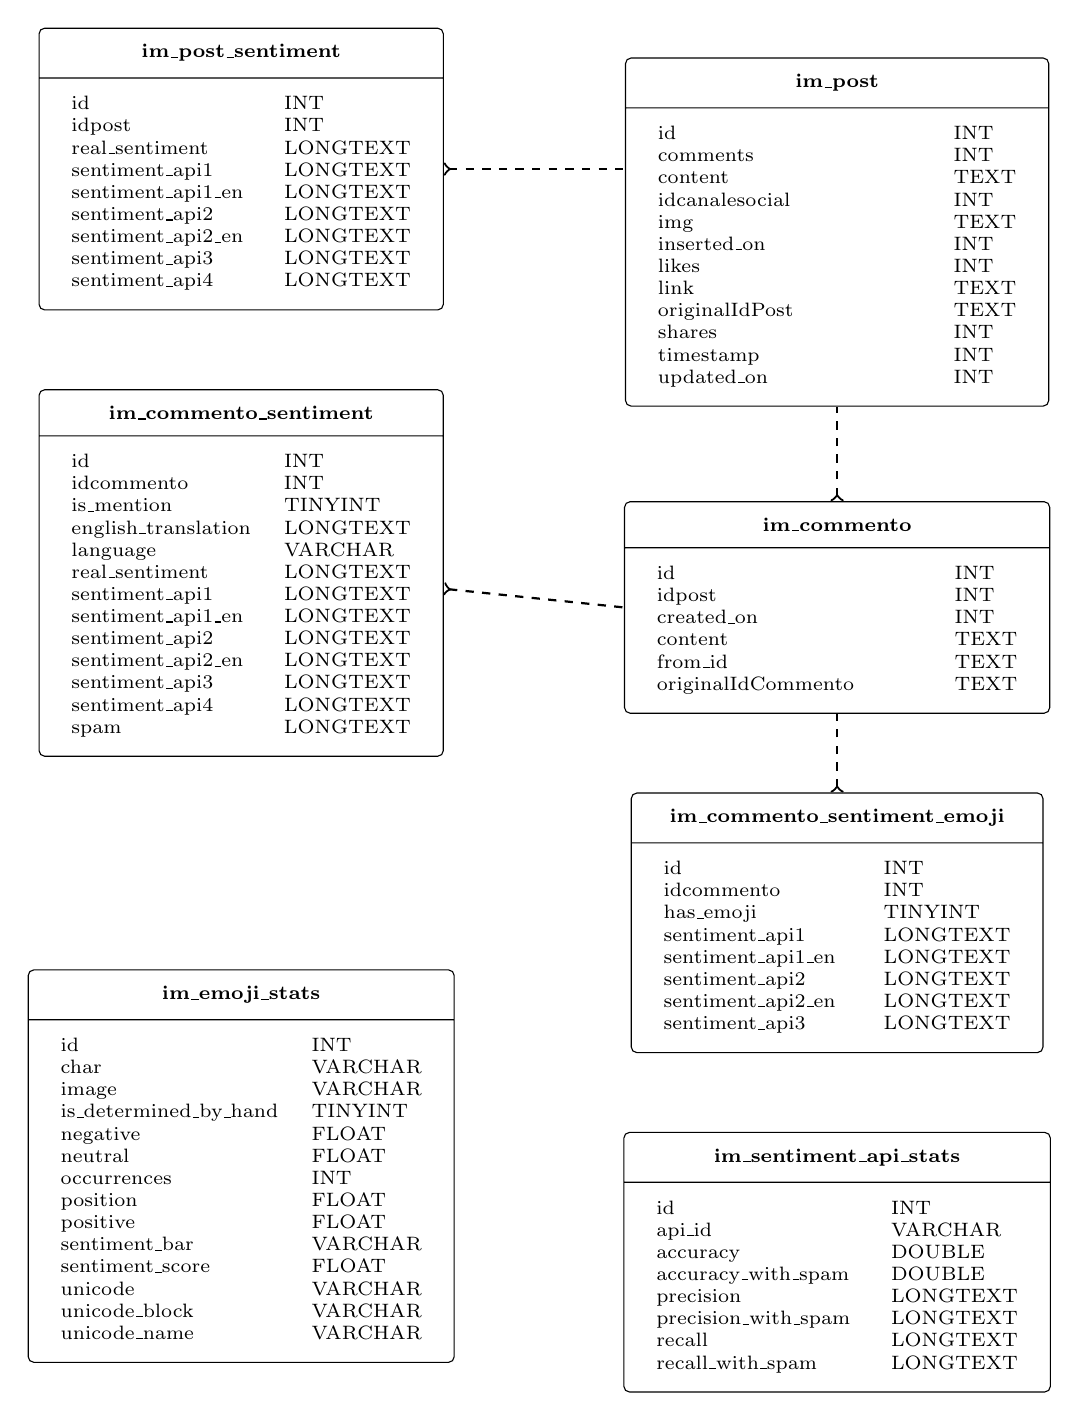
\begin{tikzpicture}[node distance=1cm]
\onehalfspacing

    \node (im-post) [table]{
        \textbf{im\_post}
        \nodepart{second}
            \tabular{ll} 
            id & INT \\ 
            comments & INT \\ 
            content & TEXT \\ 
            idcanalesocial & INT \\ 
            img & TEXT \\ 
            inserted\_on & INT \\ 
            likes & INT \\ 
            link & TEXT \\ 
            originalIdPost \ \ \ \ \ \ \ \ \ \ \ \ \ \ \ \ \ & TEXT \\
            shares & INT \\
            timestamp & INT \\
            updated\_on & INT \\                        
            \endtabular
    };

    \node (im-post-sentiment) [table, left=of im-post, yshift=0.8cm, xshift=-1.3cm]{
        \textbf{im\_post\_sentiment}
        \nodepart{second}
            \tabular{ll}                    
            id & INT \\
            idpost & INT \\
            real\_sentiment & LONGTEXT \\
            sentiment\_api1 & LONGTEXT \\
            sentiment\_api1\_en \ & LONGTEXT \\
            sentiment\_api2 & LONGTEXT \\
            sentiment\_api2\_en & LONGTEXT \\
            sentiment\_api3 & LONGTEXT \\
            sentiment\_api4 & LONGTEXT \\
            \endtabular
    };

    \node (im-commento) [table, below=of im-post,yshift=-0.2cm ]{
        \textbf{im\_commento}
        \nodepart{second}
            \tabular{ll}                    
            id & INT \\
            idpost & INT \\
            created\_on & INT \\
            content & TEXT \\
            from\_id & TEXT \\
            originalIdCommento \ \ \ \ \ \ \ \ \ & TEXT \\
            \endtabular
    };

    \node (im-commento-sentiment) [table, below=of im-post-sentiment]{
        \textbf{im\_commento\_sentiment}
        \nodepart{second}
            \tabular{ll}                    
            id & INT \\
            idcommento & INT \\
            is\_mention & TINYINT \\
            english\_translation & LONGTEXT \\
            language & VARCHAR \\
            real\_sentiment & LONGTEXT \\
            sentiment\_api1 & LONGTEXT \\
            sentiment\_api1\_en & LONGTEXT \\
            sentiment\_api2 & LONGTEXT \\
            sentiment\_api2\_en & LONGTEXT \\
            sentiment\_api3 & LONGTEXT \\
            sentiment\_api4 & LONGTEXT \\
            spam & LONGTEXT \\
            \endtabular
    };

    \node (im-commento-sentiment-emoji) [table, below=of im-commento]{
        \textbf{im\_commento\_sentiment\_emoji}
        \nodepart{second}
            \tabular{ll}                    
            id & INT \\
            idcommento & INT \\
            has\_emoji & TINYINT \\
            sentiment\_api1 & LONGTEXT \\
            sentiment\_api1\_en & LONGTEXT \\
            sentiment\_api2 & LONGTEXT \\
            sentiment\_api2\_en  \ \ & LONGTEXT \\
            sentiment\_api3 & LONGTEXT \\
            \endtabular
    };

    \node (im-sentiment-api-stats) [table, below=of im-commento-sentiment-emoji]{
        \textbf{im\_sentiment\_api\_stats}
        \nodepart{second}
            \tabular{ll}                    
            id & INT \\
            api\_id & VARCHAR \\
            accuracy & DOUBLE \\
            accuracy\_with\_spam & DOUBLE \\
            precision & LONGTEXT \\
            precision\_with\_spam \ & LONGTEXT \\
            recall & LONGTEXT \\
            recall\_with\_spam & LONGTEXT \\
            \endtabular
    };

    \node (im-emoji-stats) [table, below=of im-commento-sentiment, yshift=-1.7cm]{
        \textbf{im\_emoji\_stats}
        \nodepart{second}
            \tabular{ll}                    
            id & INT \\
            char & VARCHAR \\
            image & VARCHAR \\
            is\_determined\_by\_hand & TINYINT \\
            negative & FLOAT \\
            neutral & FLOAT \\
            occurrences & INT \\
            position & FLOAT \\
            positive & FLOAT \\
            sentiment\_bar & VARCHAR \\
            sentiment\_score & FLOAT \\
            unicode & VARCHAR \\
            unicode\_block & VARCHAR \\
            unicode\_name & VARCHAR \\
            \endtabular
    };

    \draw[line] (im-post-sentiment.east) -- ([yshift=0.8cm] im-post.west);
    \draw[line] (im-commento.north) -- (im-post.south);
    \draw[line] ([yshift=-0.2cm] im-commento-sentiment.east) -- (im-commento.west);
    \draw[line] ( im-commento-sentiment-emoji.north) |- (im-commento.south);
   
\end{tikzpicture}
  \caption{Database schema}
  \label{fig:db-schema}
\end{figure}

As previously stated, we have extended and built our framework on top of a preexisting relational MySQL database schema which came with a set of specifications which were adopted and applied to \inlinecode{sentiment\_db}.
Using a version of MySQL greater or equal to 5.5.3 was a hard constraint because in that release MySQL introduced support for \inlinecode{uft8mb4} encoding.  
As opposed to \inlinecode{uft8}'s three bytes per character maximum, 
\inlinecode{uft8mb4} uses a maximum of four bytes per character making it fully compatible with \inlinecode{uft8} and, most importantly, able to correctly encode and store emojis.
It is worth mentioning that only two data tables that were a part of the original database were used and those are \inlinecode{im\_commento} and \inlinecode{im\_post}.

For the sake of completeness, following tables contain details and field descriptions of used data tables. 

\begin{table}[H]
\centering
\onehalfspacing

\begin{tabularx}{0.95\textwidth}{ l || c | X }
	\hline
	\multicolumn{3}{l}{ \textbf{im\_post} } \\
	\hline

 	\textbf{id} & INT & PRIMARY KEY \\  
	comments & INT & number of comments the post has \\  
	content & TEXT & post's content \\  
	idcanalesocial & INT & FORGEIN KEY to im\_canalesocial: \newline field links to the post's social media account \\  
	img & TEXT & url to post's accompanying photo \\  
	inserted\_on & INT & timestamp when the record was inserted \\  
	likes & INT & number of likes the post has \\  
	link & TEXT & url to the post on a social media site \\  
	originalIdPost \ \  & TEXT & identifier used on its social media site \\ 
	shares & INT & number of shares the post has \\ 
	timestamp & INT & timestamp when the post was created \\ 
	updated\_on & INT & timestamp when the record was updated \\ 
  
	\hline
\end{tabularx}
\caption{Overview of \inlinecode{im\_post} database table}
\label{tab:im-post}

\end{table}
\begin{table}[H]
\centering
\onehalfspacing

\begin{tabularx}{0.95\textwidth}{ l || c | X }
	\hline
	\multicolumn{3}{l}{ \textbf{im\_commento} } \\
	\hline

 	\textbf{id} & INT & PRIMARY KEY \\  
	idpost & INT & FORGEIN KEY to im\_post: \newline field links to the comment's post \\  
	created\_on & INT & timestamp when the comment was created \\
	content & TEXT & comment's content \\
	from\_id & TEXT & commentator's id \\
	originalIdCommento & TEXT & identifier used on its social media site \\
 
	\hline
\end{tabularx}

\caption{Overview of \inlinecode{im\_commento} database table}
\label{tab:im-commento}

\end{table}
\newpage

As mentioned, emojis play a big role in determining sentiment of a comment. 
Since none of the APIs took them into account, we used sentiment scores from \emph{Emoji Sentiment Ranking}\footnote{http://kt.ijs.si/data/Emoji\_sentiment\_ranking} published as a part of a sentiment analysis study\cite{Kralj2015emojis},  and imported them into the database table \inlinecode{im\_emoji\_stats} whose details are shown in Table \ref{tab:im-emoji-stats}.  
However, not all emojis or emoticons that occurred in our data set were included in the study (e.g. 📘 🍾 🙂 🙄 🕶 :) :D ).
Which means they had to be manually inserted in the db. 
Their sentiment scores were determined by finding a similarly defined emoji and making the assumption that they had the same, or at least similar, sentiment. 
%All emojis that were inserted by hand are marked by a true value in  \inlinecode{is\_determined\_by\_hand} column.
For example, green book's (📗) sentiment score was used in place for the missing blue book emoji (📘). 
An example of missing inserted emojis and their similar counterparts can be found in Table \ref{tab:inserted-emoticons}
\begin{table}[H]
\centering
\onehalfspacing

\begin{tabularx}{0.95\textwidth}{ c | c | c | X }
	\hline
	\textbf{Inserted icon} & \textbf{Similar icon} & \textbf{Sentiment score} & \textbf{Unicode name} \\  
 	\hline
	📘        & 📗 & 0.491 & Blue book \\
	🙂        &  ☺ & 0.72 & Slightly smiling face \\
	🕶        & 😎 & 0.491 & Dark sunglasses \\
	:-) :) =) &  ☺ & 0.657 & Smiley face \\
	:*        & 😘 & 0.71 & Kiss face \\
\textless3    & ❤  &  0.657 & Heart  \\
	\hline
\end{tabularx}

\caption{Example of inserted emojis into \inlinecode{im\_emoji\_stats} database table}
\label{tab:inserted-emoticons}

\end{table}
\begin{table}[H]
\centering
\onehalfspacing

\begin{tabularx}{0.95\textwidth}{ l || c | X }
	\hline
	\multicolumn{3}{l}{ \textbf{im\_emoji\_stats} } \\
	\hline
 	\textbf{id} & INT & PRIMARY KEY \\  
	char & VARCHAR &  emoji  characers \\ 
	is\_determined\_by\_hand & TINYINT & boolean variable that denotes if emoji or emoticons were added by hand or used stats from the study \emph{Emoji Sentiment Ranking} \\ 
	negative & FLOAT &  how negative is the emoji $\in [0,1]$ \\ 
	neutral & FLOAT &  how neutral is the emoji $\in [0,1]$ \\ 
	occurrences & INT & number of occurrences of the emoji in all comments in our dataset \\ 
	positive & FLOAT & how positive is the emoji $\in [0,1]$ \\ 
	sentiment\_score & FLOAT & overall sentiment score $\in [-1,1]$ \\ 
	unicode & VARCHAR & unicode codepoint of the emoji \\ 
	unicode\_block & VARCHAR & general category an emoji falls into \\ 
	unicode\_name & VARCHAR & descriptive name of the emoji \\ 
	\hline
\end{tabularx}

\caption{Overview of \inlinecode{im\_emoji\_stats} database table}
\label{tab:im-emoji-stats}

\end{table}

Tables \ref{tab:im-commento-sentiment}, \ref{tab:im-post-sentiment}, \ref{tab:im-commento-sentiment} and \ref{tab:im-sentiment-api-stats}  

Why json when it violated the 1NN rule? already in mysql, will eventually support json, and easily movable to nosql db, or even elastic search. 

Out of the table columns listed above, the following are in json format but stored as lontext:



\newsavebox\sentimentexample
\newsavebox\spamexample

\begin{lrbox}{\sentimentexample}
\begin{lstlisting}[
style=json,
label={lst:default-sentiment-json-table}]
{
  "sentiment_label": "",
  "sentiment_stats": {
      "positive": 0,
      "negative": 0
      "neutral" : 0
  }
}
\end{lstlisting}
\end{lrbox}

\begin{lrbox}{\spamexample}
\begin{lstlisting}[
style=json,
label={lst:default-spam-json}]
{
  "type": "", 
  "is_spam": false
}
\end{lstlisting}
\end{lrbox}

\begin{table}[H]
\centering
\onehalfspacing

\begin{tabularx}{0.95\textwidth}{ m{35mm} || c | X }
	\hline
	\multicolumn{3}{l}{ \textbf{im\_commento\_sentiment / im\_commento\_sentiment\_emoji} } \\ \hline
	\hline
	\textbf{id} & INT & PRIMARY KEY \\ \hline  
    idcommento & INT & FORGEIN KEY to im\_comment: \newline the field points to comment's id \\ \hline  
    is\_mention & TINYINT & boolean variable that denotes if there was a mention of a user in the comment (e.q @Anna) \\ \hline  
    english\_translation & LONGTEXT & Google Translate API's English translation of the content \\ \hline
    language & VARCHAR & Google Translate API's prediction of content's  original language \\ \hline
	real\_sentiment & LONGTEXT & manually determined sentiment\\ \hline
	sentiment\_api1,
	sentiment\_api1\_en, 
	sentiment\_api2, 
	sentiment\_api2\_en,
	sentiment\_api3, 
	sentiment\_api4 & LONGTEXT & 
	\begin{tabular}[t]{ m{60mm}}
		API's sentiment prediction of content in original (English) language. 
		All \inlinecode{sentiment\_api} columns default to:\newline
		\usebox\sentimentexample  
  	\end{tabular}\\ \hline
	spam & LONGTEXT & manually determined whether or not the content is spam\newline defaults to:\newline
\usebox\spamexample  \\ \hline

\end{tabularx}
\caption{Overview of \inlinecode{im\_commento\_sentiment} and \newline \inlinecode{im\_commento\_sentiment\_emoji} database table}
\label{tab:im-commento-sentiment}

\end{table}
\newsavebox\postsentimentexample

\begin{lrbox}{\postsentimentexample}
\begin{lstlisting}[
style=json,
label={lst:default-post-sentiment-json}]
{
  "sentiment_stats": {
    "positive": 9, 
    "negative": 2,
    "neutral": 38, 
    "total": 49
  }, 
  "sentiment_label": "neutral"
  "total_comments": 49,
}
\end{lstlisting}
\end{lrbox}


\begin{table}[H]
\centering
\onehalfspacing

\begin{tabularx}{0.95\textwidth}{ m{35mm} || c | X }
	\hline
	\multicolumn{3}{l}{ \textbf{im\_post\_sentiment} } \\ \hline
	\hline
	\textbf{id} & INT & PRIMARY KEY \\ \hline  
    idpost & INT & FORGEIN KEY to im\_post: \newline the field points to post's id \\ \hline  
    real\_sentiment & LONGTEXT & aggregation over post's comments of: real sentiment data \\ \hline 
	sentiment\_api1,
	sentiment\_api1\_en, 
	sentiment\_api2, 
	sentiment\_api2\_en,
	sentiment\_api3, 
	sentiment\_api4 & LONGTEXT & 
	\begin{tabular}[t]{ m{60mm}}
		aggregation over post's comments of:
		API's sentiment predictions in original (English) language.
		All \inlinecode{sentiment\_api} columns default to:\newline
		\usebox\postsentimentexample 
  	\end{tabular}\\ \hline


\end{tabularx}
\caption{Overview of \inlinecode{im\_post\_sentiment} database table}
\label{tab:im-post-sentiment}

\end{table}
\newsavebox\sentimentstatsexample
\newsavebox\apiid

\begin{lrbox}{\apiid}
\begin{lstlisting}[
style=json,
label={lst:api-id-json}]
 sentiment_api1, 
 sentiment_api1_en, 
 sentiment_api1_emoji,
 sentiment_api1_en_emoji,
 sentiment_api2 ...
\end{lstlisting}
\end{lrbox}


\begin{lrbox}{\sentimentstatsexample}
\begin{lstlisting}[
style=json,
label={lst:sentiment-api-stats-json}]
{
  "positive": 0.5965, 
  "negative": 0.3946,
  "neutral":  0.4578 
}
\end{lstlisting}
\end{lrbox}


\begin{table}[H]
\centering
\onehalfspacing

\begin{tabularx}{0.95\textwidth}{ l || c | X }
	\hline
	\multicolumn{3}{l}{ \textbf{im\_sentiment\_api\_stats} } \\ \hline
	\hline

	\textbf{id} & INT & PRIMARY KEY \\ \hline 
	api\_id & VARCHAR & String identifying API and comment content version used. For example: \newline \usebox\apiid
	 \\ \hline  
    accuracy & DOUBLE & Accuracy of the API excluding comments marked as spam \\ \hline  
    accuracy\_with\_spam & DOUBLE & Accuracy of the API including comments marked as spam \\ \hline 
    
    precision & LONGTEXT & Precision per sentiment label of the API excluding comments marked as spam \\ \hline 
	precision\_with\_spam & LONGTEXT & Precision per sentiment label of the API including comments marked as spam \\ \hline

	recall & LONGTEXT & Recall per sentiment label of the API excluding comments marked as spam \\ \hline 
	recall\_with\_spam & LONGTEXT & Recall per sentiment label of the API including comments marked as spam \newline
	Example of recall and precision column values:\newline
	\usebox\sentimentstatsexample  \\ \hline

\end{tabularx}
\caption{Overview of \inlinecode{im\_sentiment\_api\_stats} database table}
\label{tab:im-sentiment-api-stats}

\end{table}

% --- SENTIMENT ANALYSIS APIS --
\newcommand*{\APIsOverviewPath}{04-framework/02-implementation/02-apis}

\subsection{Sentiment analysis APIs\label{sec:apis}}
Each of the APIs is called by making a either a HTTP or HTTPS post request with a specific payload. The responses vary but all are parsed and stored in the format like the one shown in Listing \ref{lst:default-sentiment-json}.

\subsubsection*{Vivekn API}

\begin{description}
\singlespacing
 \item[Author:] Vivek Narayanan
 \item[Web url:] http://sentiment.vivekn.com/docs/api/
 \item[Database columns:] \inlinecode{sentiment\_api1} and \inlinecode{sentiment\_api1\_en}
\end{description}
As described on the API's website, the tool works by examining individual words and short sequences of words which it then compares against a probability model. The probability model was built on a prelabeled test set of IMDb movie reviews
and it is based on the \emph{Fast and accurate sentiment classification using an enhanced Naive Bayes model} study \cite{DBLP:journals/corr/abs-1305-6143}.
The API is invoked via an HTTP post request with a \inlinecode{txt} payload that supplies comment's content. 
The request, response and the form in which the response was stored in \inlinecode{sentiment\_db} is presented in Table \ref{tab:vivekn-api}.

\newsavebox\vivekresponse
\newsavebox\viveknrequest
\newsavebox\vivekndb

\begin{lrbox}{\viveknrequest}
\begin{lstlisting}[style=json]
{  
  "txt": "Beautiful!" 
}
\end{lstlisting}
\end{lrbox}


\begin{lrbox}{\vivekresponse}
\begin{lstlisting}[style=json]
{ 
  "result": { 
    "sentiment": "Positive", 
    "confidence" : 72.422451 
  } 
}
\end{lstlisting}
\end{lrbox}

\begin{lrbox}{\vivekndb}
\begin{lstlisting}[style=json]
{
  "sentiment_label": "positive",
  "sentiment_stats": {
      "positive": 0.724,
      "negative": 0,
      "neutral" : 0
  }
}
\end{lstlisting}
\end{lrbox}

\begin{table}[H]
\centering
\singlespacing

\begin{tabularx}{0.9\textwidth}{ m{30mm}  X }
\hline  
  \textbf{request}  & \usebox\viveknrequest \\ \hline  
  \textbf{response} & \usebox\vivekresponse  \\ \hline  
  \textbf{stored} & \usebox\vivekndb  \\ \hline  

\end{tabularx}
\caption{Request and response payload to Vivekn API}
\label{tab:vivekn-api}

\end{table}


\subsubsection*{Text-processing API}
\begin{description}
\singlespacing
 \item[Web url:] http://text-processing.com/docs/sentiment.html
 \item[Database columns:] \inlinecode{sentiment\_api2} and \inlinecode{sentiment\_api2\_en}
\end{description}
This API is also trained on movie reviews but uses two binary classifiers. More specifically, it uses hierarchical classification by combining a subjectivity classifier and a polarity classifier. First, the subjectivity classifier determines whether the text is objective or subjective. If the text is objective, then it is classified as neutral. Otherwise the polarity classifier is used to determine if the text is positive or negative.  More details on the implementation can be found in articles  \cite{NaiveBayes}, \cite{Stopwords}, \cite{LowInformationFeatures} and \cite{HierarchicalClassification}.
However, the two classifier model introduces a caveat. Sentiment probabilities of positive and negative labels always sum up to one, while the neutral label is standalone and dominates the result if its probability is greater than 0.5.
The response, request and the stored JSON strings are shown in Table \ref{tab:text-processing-api}.
\newsavebox\tpresponse
\newsavebox\tprequest
\newsavebox\tpdb

\begin{lrbox}{\tprequest}
\begin{lstlisting}[style=json]
{  
  "text": "Beautiful!" 
}
\end{lstlisting}
\end{lrbox}


\begin{lrbox}{\tpresponse}
\begin{lstlisting}[style=json]
{
  "label": "neg",
  "probability": {
    "neutral": 0.38637609994709854,
    "neg": 0.68846305481785608,
    "pos": 0.31153694518214375
  }
}
\end{lstlisting}
\end{lrbox}

\begin{lrbox}{\tpdb}
\begin{lstlisting}[style=json]
{
  "sentiment_label": "negative",
  "sentiment_stats": {
      "positive": 0.311,
      "negative": 0.688,
      "neutral" : 0.386
  }
}
\end{lstlisting}
\end{lrbox}

\begin{table}[H]
\centering
\singlespacing

\begin{tabularx}{0.9\textwidth}{ m{30mm}  X }
\hline  
  \textbf{request}  & \usebox\tprequest \\ \hline  
  \textbf{response} & \usebox\tpresponse  \\ \hline  
  \textbf{stored} & \usebox\tpdb  \\ \hline  

\end{tabularx}
\caption{Request and response payload to Text-processing API}
\label{tab:text-processing-api}

\end{table}

\newpage

\subsubsection*{Indico API}
\begin{description}
\singlespacing
 \item[Web url:] https://indico.io/docs\#sentiment 
 \item[Web url (hq):] https://indico.io/docs\#sentiment\_hq 
 \item[Database columns:] \inlinecode{sentiment\_api3} and \inlinecode{sentiment\_api4 (hq)}
\end{description}
Even though we used all APIs as black boxes, the Indico API was treated as such even more so because implementation details weren't readily available on its website. 
It was also the only API that required registration in order to obtain an authorization key to access it. 
It did, however, provide two different endpoints, a regular sentiment analysis and a high quality (hq) version.
API's response is a number between 0 and 1. 
This number represents the likelihood that the analyzed text is positive. 
Meaning, values greater than 0.5 indicate positive sentiment, while values below that threshold indicate a negative sentiment. 
Since we were operating within a three label domain, a script was made to label all likelihoods $\in[a,b]$ as neutral to see how the accuracy (and other metrics) would change.
The response, request and the stored JSON are listed in Table \ref{tab:indico-api}.

\newsavebox\indicoresponse
\newsavebox\indicorequest
\newsavebox\indicodb

\begin{lrbox}{\indicorequest}
\begin{lstlisting}[style=json]
{  
  "text": "Beautiful!" 
}
\end{lstlisting}
\end{lrbox}


\begin{lrbox}{\indicoresponse}
\begin{lstlisting}[
style=json,
label={lst:indico-json}]
{
  "results": 0.3468102081511113
}
\end{lstlisting}
\end{lrbox}

\begin{lrbox}{\indicodb}
\begin{lstlisting}[style=json]
{
  "sentiment_label": "positive",
  "sentiment_stats": {
      "positive": 0.654,
      "negative": 0.346,
      "neutral" : 0
  }
}
\end{lstlisting}
\end{lrbox}

\begin{table}[H]
\centering
\singlespacing

\begin{tabularx}{0.9\textwidth}{ m{30mm}  X }
\hline  
  \textbf{request}  & \usebox\indicorequest \\ \hline  
  \textbf{response} & \usebox\indicoresponse  \\ \hline  
  \textbf{stored} & \usebox\indicodb  \\ \hline  

\end{tabularx}
\caption{Request and response payload to Indico and IndicoHq API endpoints}
\label{tab:indico-api}

\end{table}


% --- SUBSECTION SCRIPTS ---
\subsection{Sentiment analysis scripts\label{sec:sentiment-analysis-workflow}}

The logic of all workflows described in Chapter \ref{ch:sentiment-analysis-workflow} are implemented as a collection of python scripts.
If we were to take the top down approach as we did in Chapter \ref{ch:sentiment-analysis-workflow}, we can start identifying specific nodes in workflow flowcharts to single scripts.

Predicting sentiment, determining real sentiment and the prediction evaluation parts of Figure \ref{fig:analysis-workflow} are realized via 
\emph{\wrapunderscore{automated\_sentiment\_analysis.py}}, 
\emph{\wrapunderscore{update\_real\_sentiment\_and\_spam.py}} and 
\emph{\wrapunderscore{evaluate\_api\_performance.py}}, respectively.

% -- API EVALUATION --
\subsubsection*{API evaluation script}
\noindent The \emph{\wrapunderscore{evaluate\_api\_performance.py}}\ script can be evoked via the command line and it stores the results in \inlinecode{im\_sentiment\_api\_stats} database table. It accepts the following optional arguments:

\begin{description}[labelindent=0.7cm, leftmargin=1.7cm]
\singlespacing
\item[--help ] shows all available arguments and exits
\item[--api \textless name\textgreater] 
	specifies which API $\in$ \lcb 
	sentiment\_api1, 
	sentiment\_api1\_en, 
	sentiment\_api2, 
	sentiment\_api2\_en, 
	sentiment\_api3, 
	sentiment\_api4\rcb\ to evaluate. If not specified, script evaluates all APIs 
\item[--metric \textless name\textgreater ] specifies which
	specifies which metric $\in$ \lcb
	precision, accuracy, recall\rcb\ to calculate. If not specified, script calculates all metrics
\item[--spam] calculates performance metric(s) for specified API(s) taking into consideration all comments regardless weather or non they were tagged as spam
\item[--no-spam] calculates performance metric(s) for specified API(s) taking into consideration only the comments not tagged as spam. 
If neither \inlinecode{no-spam} nor \inlinecode{spam} arguments were specified, the metrics are calculated for both cases
\item[--emoji] calculates performance metric(s) for specified API(s) of sentiment statistics that accounted for emojis. 
\item[--no-emoji] calculates performance metric(s) for specified API(s) of sentiment statistics that didn't accounted for emojis. 
If neither \inlinecode{no-emoji} nor \inlinecode{emoji} arguments were specified, the metrics are calculated for both cases
\end{description}
\textbf{Usage and sample output}


\begin{verbatim}
$ python evaluate_api_performance.py --metric accuracy --emoji --spam
----------------------------------------------------
Calculations for api: sentiment_api1_emoji with spam
Real sentiment distribution {
  "positive": "43.51%", 
  "neutral": "45.61%", 
  "negative": "10.88%"
}
True positives: {'positive': 1205, 'neutral': 2167, 'negative': 177} 
False negatives: {'positive': 1439, 'neutral': 605, 'negative': 484} 
False positives: {'positive': 517, 'neutral': 1694, 'negative': 317} 
Total sentiment predictions: 6077 
Accuracy: 0.584000 
- - - - - - - - - - - - - - - - - - - - - - - - - -
Updating table im_sentiment_api_stats
Setting `accuracy_with_spam` = 0.584 
Where `api_id` = 'sentiment_api1_emoji' 
... 1 row affected
----------------------------------------------------
\end{verbatim}


% -- REAL SENTIMENT --
\subsubsection*{Script for determining real sentiment}
\noindent The \emph{\wrapunderscore{update\_real\_sentiment\_and\_spam.py}} script can be evoked via the command line and stores the results in \.
For each comment the script displays its content and prompts user for input to determine: 
 \begin{enumerate}
  \item whether or not the comment is only a user tag (e.g @Anna)
  \item whether or not the comment is spam and if so, to specify a type
  \item comment sentiment
\end{enumerate}
The script accepts the following optional arguments:
\begin{description}[labelindent=0.7cm, leftmargin=1.7cm]
\singlespacing
 \item[--help ] shows all available arguments and exits
 \item[-ideq \textless nbs\textgreater ] specifies ids of the comments for which \\ we want to determine the real sentiment
 \item[-idgt \textless nb\textgreater] gets all comments that satisfy $id > nb$
 \item[-idlt \textless nb\textgreater] gets all comments that satisfy $id < nb$
\end{description}
\textbf{Usage and sample output}

\begin{verbatim}
$  python update_real_sentiment_and_spam.py -ideq 6
--------------------------------------------------
Comment_id: 6
Content: Bellissime!
English translation: Beautiful!
- - - - - - - - - - - - - - - - - - - - - - - - - 
Is this comment ONLY a mention? (y/n): n
Updating table im_commento_sentiment
Setting `is_mention` = '0' 
Where idcommento = 6 
... 1 row affected
- - - - - - - - - - - - - - - - - - - - - - - - - 
Is this comment spam? (y/n): n
Updating table im_commento_sentiment
Setting `spam` = '{"type": "", "is_spam": false}' 
Where idcommento = 6 
... 1 row affected
- - - - - - - - - - - - - - - - - - - - - - - - - 
Determine the real_sentiment:
pos/neg/neu/mix? pos
Updating table im_commento_sentiment
Setting `real_sentiment` = '{
  "sentiment_stats": {
    "positive": 1, 
    "neutral": 0, 
    "negative": 0
  }, 
  "sentiment_label": "positive"
}'
Where idcommento = 6 
... 1 row affected
--------------------------------------------------
\end{verbatim}






% --- SUBSECTION WEB SERVER ---
\subsection{Web server}\label{sec:web-server}

Our application is hosted on Digital ocean droplet, connected to domain name \textit{sentiment-analysis.ml}. Underneath the framework lays a Linux Ubuntu virtual machine with 512MB of RAM memory, 20GB of disk space.

Web application follows Django Model Template View pattern, from now on reffered as MTV, which is similar to Model View Controller pattern. In MTV pattern the \textit{view} sort of plays the role of a controller. In Django’s interpretation of MVC, the view describes the data that gets presented to the user; it’s not necessarily just how the data looks, but which data is presented which has been explained more in depth in Mastering Django: Core\cite{DjangoMTV}. The Model in MTV represents the data access layer, which contains features related to the data: how to access it, how to validate it, which behaviors it has, and the relationships between the data. The Template in MTV is the presentation layer. This layer contains way of representing data in the web page. The View in MTV is the business logic layer. This layer contains the logic that accesses the model and connect it to the one of the templates. Views are usually positioned between models and templates.

Part of our framework's GUI is based on Django REST API which provides a handy way of interacting with the data. For example, providing a default GUI for adding, deleting and editing data. Other than being able to access the API via a browser, it can also be done from the command-line, using tools like curl.
\newpage